\documentclass[11pt]{memoir}

\usepackage{importationsprojet}
\pagestyle{empty}
\newgeometry{margin=1cm}

\newenvironment{centre}
 {\parskip=0pt\par\nopagebreak\centering}
 {\par\noindent\ignorespacesafterend}

\begin{document}
\begin{questions}

\exercicetitre{Nombres mixte} 

Décomposer les fractions suivantes en la somme d'un nombre entier et d'une fraction comprise entre 0 et 1.

\begin{multicols}{6}
    \questionX $\dfrac{17}{8}=$
    \questionX $\dfrac{24}{7}=$
    \questionX $\dfrac{77}{3}=$
    \questionX $\dfrac{83}{9}=$
    \questionX $\dfrac{17}{4}=$
    \questionX $\dfrac{27}{5}=$
\end{multicols}

\exercicetitre{Encadrement de fractions}

Encadrer les fractions suivantes par deux entiers successifs.

\begin{multicols}{6}
    \questionX $~~~<\dfrac{77}{8}<$
    \questionX $~~~<\dfrac{83}{7}<$
    \questionX $~~~<\dfrac{17}{3}<$
    \questionX $~~~<\dfrac{24}{9}<$
    \questionX $~~~<\dfrac{27}{4}<$
    \questionX $~~~<\dfrac{17}{5}<$
\end{multicols}

\exercicetitre{Diviseurs}

\question Compléter le tableau suivant.

\begin{centre}
\begin{tabularx}{0.6\linewidth}{|c|C|C|C|C|C|}\hline
    ... est divisible par & 2 & 3 & 5 & 9 & 10 \\\hline
    5912 & & & & & \\\hline
    34200 & & & & & \\ \hline
    54208 & & & & & \\ \hline
    317 & & & & & \\ \hline
    708 & & & & & \\ \hline
     & non & oui & non & non & non \\\hline
     & oui & oui & non & oui & non \\\hline
     & non & oui & oui & non & non \\\hline
     & oui & oui & oui & oui & oui \\\hline
     & non & non & non & non & non \\\hline
\end{tabularx}
\end{centre}

\exercicetitre{Représentation graphique} 

Sur le site de Météo France, il est possible de recueillir les données météorologiques liées à une ville, comme Crécy-la-Chapelle par exemple. Intéressons-nous à la moyenne mensuelle des précipitations sur les données recueillies entre 1995 et 2010. \\(\textit{les données ont été arrondies au millimètre})

\begin{centre}
\begin{tabularx}{0.9\linewidth}{|l||*{12}{C|}}\hline
    Mois & jan. & fév. & mars & avril & mai & juin & juil. & août & sept. & oct. & nov. & déc. \\\hline
    Précipitations (\unit{\milli\meter}) & 52 &  & 50 & 50 & 59 &  & 66 & 69 & 49 &  & 61 & 62 \\\hline
\end{tabularx}
\end{centre}

\begin{centre}
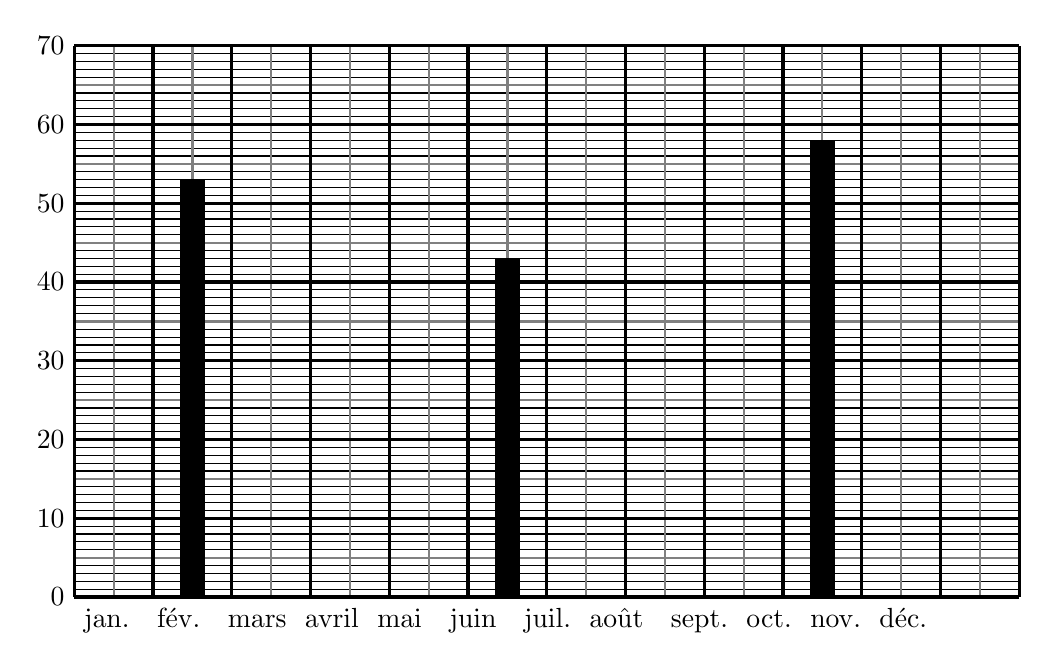
\begin{tikzpicture}
    \draw (0,0) grid[ystep=0.1] (12,7);
    \draw[gray, thick] (0,0) grid[step=0.5] (12,7);
    \draw[very thick] (0,0) grid[step=1] (12,7);
    \node[right] at (0,-0.3) {jan.~~~fév.~~~mars~~avril~~mai~~~juin~~~juil.~~août~~~sept.~~oct.~~nov.~~déc.};
    \foreach \x in {0,10,...,70} { \node[left] at (0,\x/10) {\x}; }
    \draw[fill=black] (5.35,0) rectangle (5.65,4.3);
    \draw[fill=black] (9.35,0) rectangle (9.65,5.8);
    \draw[fill=black] (1.35,0) rectangle (1.65,5.3);
\end{tikzpicture}
\end{centre}

\question Compléter le tableau et le diagramme en barres, sachant qu'ils représentent le même jeu de données.
\question Interpréter les résultats.

\clearpage

\exercicetitre{Calculs avec priorités}
    \question $7 \times  3 + 4$
    \question $(9+3) \times (1+2)$
    \question $7 + 9 \times 4 + 3$
    \question $3 + 3 \times 6 \div 2$
    \question $3 \times \left[ 87 - \left( 30 + 55 \right) \right]$

\exercicetitre{Somme ou produit ?}\vspace{-2em}
    \begin{multicols}{3}
        \question $8x+5$
        \question $3x(7x-5)$
        \question $(4\alpha - 2)^2$
        \question $9x^2+5x+1$
        \question $7(x+3) + 6x$
        \question $(4x+2)(6x+1)$
    \end{multicols}

\exercicetitre{Symétries}
    \question Construire un carré $ABCD$ de côté \qty{4}{\centi\metre}.
    \question Construire tous les axes de symétries dans ce carré.
    \question Construire un losange $EFGH$ de côté \qty{4}{\centi\metre} et tel que $\widehat{EFG} = \ang{120}$.
    \question Construire le symétrique de $EFGH$ par rapport au point $H$.

\exercicetitre{}

\end{questions}
\end{document}


